% Created by tikzDevice version 0.12.4 on 2023-11-07 16:59:25
% !TEX encoding = UTF-8 Unicode
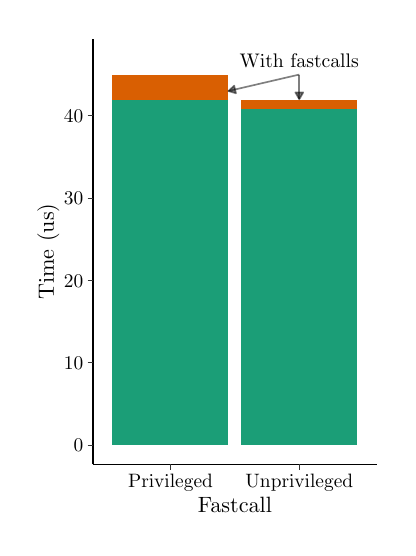
\begin{tikzpicture}[x=1pt,y=1pt]
\definecolor{fillColor}{RGB}{255,255,255}
\path[use as bounding box,fill=fillColor,fill opacity=0.00] (0,0) rectangle (130.09,180.67);
\begin{scope}
\path[clip] (  0.00,  0.00) rectangle (130.09,180.67);
\definecolor{drawColor}{RGB}{255,255,255}
\definecolor{fillColor}{RGB}{255,255,255}

\path[draw=drawColor,line width= 0.4pt,line join=round,line cap=round,fill=fillColor] (  0.00,  0.00) rectangle (130.09,180.68);
\end{scope}
\begin{scope}
\path[clip] ( 23.66, 22.85) rectangle (126.09,176.67);
\definecolor{fillColor}{RGB}{255,255,255}

\path[fill=fillColor] ( 23.66, 22.85) rectangle (126.09,176.67);
\definecolor{fillColor}{RGB}{217,95,2}

\path[fill=fillColor] ( 30.65,154.42) rectangle ( 72.55,163.66);
\definecolor{fillColor}{RGB}{27,158,119}

\path[fill=fillColor] ( 30.65, 29.84) rectangle ( 72.55,154.42);
\definecolor{fillColor}{RGB}{217,95,2}

\path[fill=fillColor] ( 77.20,151.31) rectangle (119.10,154.52);
\definecolor{fillColor}{RGB}{27,158,119}

\path[fill=fillColor] ( 77.20, 29.84) rectangle (119.10,151.31);
\definecolor{drawColor}{RGB}{0,0,0}

\path[draw=drawColor,draw opacity=0.50,line width= 0.6pt,line join=round] ( 72.55,157.78) -- ( 98.15,163.73);
\definecolor{fillColor}{RGB}{0,0,0}

\path[draw=drawColor,draw opacity=0.50,line width= 0.6pt,line join=round,fill=fillColor,fill opacity=0.50] ( 74.62,159.72) --
	( 72.55,157.78) --
	( 75.27,156.95) --
	cycle;

\path[draw=drawColor,draw opacity=0.50,line width= 0.6pt,line join=round] ( 98.15,154.81) -- ( 98.15,163.73);

\path[draw=drawColor,draw opacity=0.50,line width= 0.6pt,line join=round,fill=fillColor,fill opacity=0.50] ( 96.73,157.27) --
	( 98.15,154.81) --
	( 99.58,157.27) --
	cycle;
\definecolor{drawColor}{RGB}{0,0,0}

\node[text=drawColor,anchor=base,inner sep=0pt, outer sep=0pt, scale=  0.71] at ( 98.15,166.18) {With fastcalls};
\end{scope}
\begin{scope}
\path[clip] (  0.00,  0.00) rectangle (130.09,180.67);
\definecolor{drawColor}{RGB}{0,0,0}

\path[draw=drawColor,line width= 0.6pt,line join=round] ( 23.66, 22.85) --
	( 23.66,176.67);
\end{scope}
\begin{scope}
\path[clip] (  0.00,  0.00) rectangle (130.09,180.67);
\definecolor{drawColor}{RGB}{0,0,0}

\node[text=drawColor,anchor=base east,inner sep=0pt, outer sep=0pt, scale=  0.70] at ( 20.06, 27.43) {0};

\node[text=drawColor,anchor=base east,inner sep=0pt, outer sep=0pt, scale=  0.70] at ( 20.06, 57.18) {10};

\node[text=drawColor,anchor=base east,inner sep=0pt, outer sep=0pt, scale=  0.70] at ( 20.06, 86.94) {20};

\node[text=drawColor,anchor=base east,inner sep=0pt, outer sep=0pt, scale=  0.70] at ( 20.06,116.69) {30};

\node[text=drawColor,anchor=base east,inner sep=0pt, outer sep=0pt, scale=  0.70] at ( 20.06,146.44) {40};
\end{scope}
\begin{scope}
\path[clip] (  0.00,  0.00) rectangle (130.09,180.67);
\definecolor{drawColor}{gray}{0.20}

\path[draw=drawColor,line width= 0.4pt,line join=round] ( 21.66, 29.84) --
	( 23.66, 29.84);

\path[draw=drawColor,line width= 0.4pt,line join=round] ( 21.66, 59.59) --
	( 23.66, 59.59);

\path[draw=drawColor,line width= 0.4pt,line join=round] ( 21.66, 89.35) --
	( 23.66, 89.35);

\path[draw=drawColor,line width= 0.4pt,line join=round] ( 21.66,119.10) --
	( 23.66,119.10);

\path[draw=drawColor,line width= 0.4pt,line join=round] ( 21.66,148.85) --
	( 23.66,148.85);
\end{scope}
\begin{scope}
\path[clip] (  0.00,  0.00) rectangle (130.09,180.67);
\definecolor{drawColor}{RGB}{0,0,0}

\path[draw=drawColor,line width= 0.6pt,line join=round] ( 23.66, 22.85) --
	(126.09, 22.85);
\end{scope}
\begin{scope}
\path[clip] (  0.00,  0.00) rectangle (130.09,180.67);
\definecolor{drawColor}{gray}{0.20}

\path[draw=drawColor,line width= 0.4pt,line join=round] ( 51.60, 20.85) --
	( 51.60, 22.85);

\path[draw=drawColor,line width= 0.4pt,line join=round] ( 98.15, 20.85) --
	( 98.15, 22.85);
\end{scope}
\begin{scope}
\path[clip] (  0.00,  0.00) rectangle (130.09,180.67);
\definecolor{drawColor}{RGB}{0,0,0}

\node[text=drawColor,anchor=base,inner sep=0pt, outer sep=0pt, scale=  0.70] at ( 51.60, 14.43) {Privileged};

\node[text=drawColor,anchor=base,inner sep=0pt, outer sep=0pt, scale=  0.70] at ( 98.15, 14.43) {Unprivileged};
\end{scope}
\begin{scope}
\path[clip] (  0.00,  0.00) rectangle (130.09,180.67);
\definecolor{drawColor}{RGB}{0,0,0}

\node[text=drawColor,anchor=base,inner sep=0pt, outer sep=0pt, scale=  0.80] at ( 74.87,  5.56) {Fastcall};
\end{scope}
\begin{scope}
\path[clip] (  0.00,  0.00) rectangle (130.09,180.67);
\definecolor{drawColor}{RGB}{0,0,0}

\node[text=drawColor,rotate= 90.00,anchor=base,inner sep=0pt, outer sep=0pt, scale=  0.80] at (  9.51, 99.76) {Time (us)};
\end{scope}
\end{tikzpicture}
